\section{Dataset Statistics and Release QA}
\label{sec:stats}

This section summarizes the canonical CARScenes v1 release rather than the raw annotation dump. Every count reported here is derived from the generated release artifacts in \texttt{release/carscenes-v1/}.

\subsection{Source Composition}

\begin{table}[t]
    \centering
    \caption{Canonical CARScenes v1 split sizes by source.}
    \label{tab:split}
    \begin{tabular}{lccc}
        \toprule
        Source & Train & Silver-dev & Audit cand. \\
        \midrule
        Argoverse1 & 684 & 125 & 25 \\
        Cityscapes & 445 & 125 & 25 \\
        KITTI & 599 & 125 & 25 \\
        nuScenes & 2\,864 & 125 & 25 \\
        \midrule
        Total & 4\,592 & 500 & 100 \\
        \bottomrule
    \end{tabular}
\end{table}

Figure~\ref{fig:dataset-attributes} summarizes the marginal distributions of common scalar fields. Figure~\ref{fig:dataset-severity} visualizes the severity histogram over the full canonical release. The release contains \textbf{3,120} low-severity records (\(1{-}3\)), \textbf{1,914} mid-severity records (\(4{-}6\)), and \textbf{158} high-severity records (\(7{-}10\)). The median severity is \textbf{3}, with interquartile range \textbf{[2, 4]}.

\begin{figure*}[t]
    \centering
    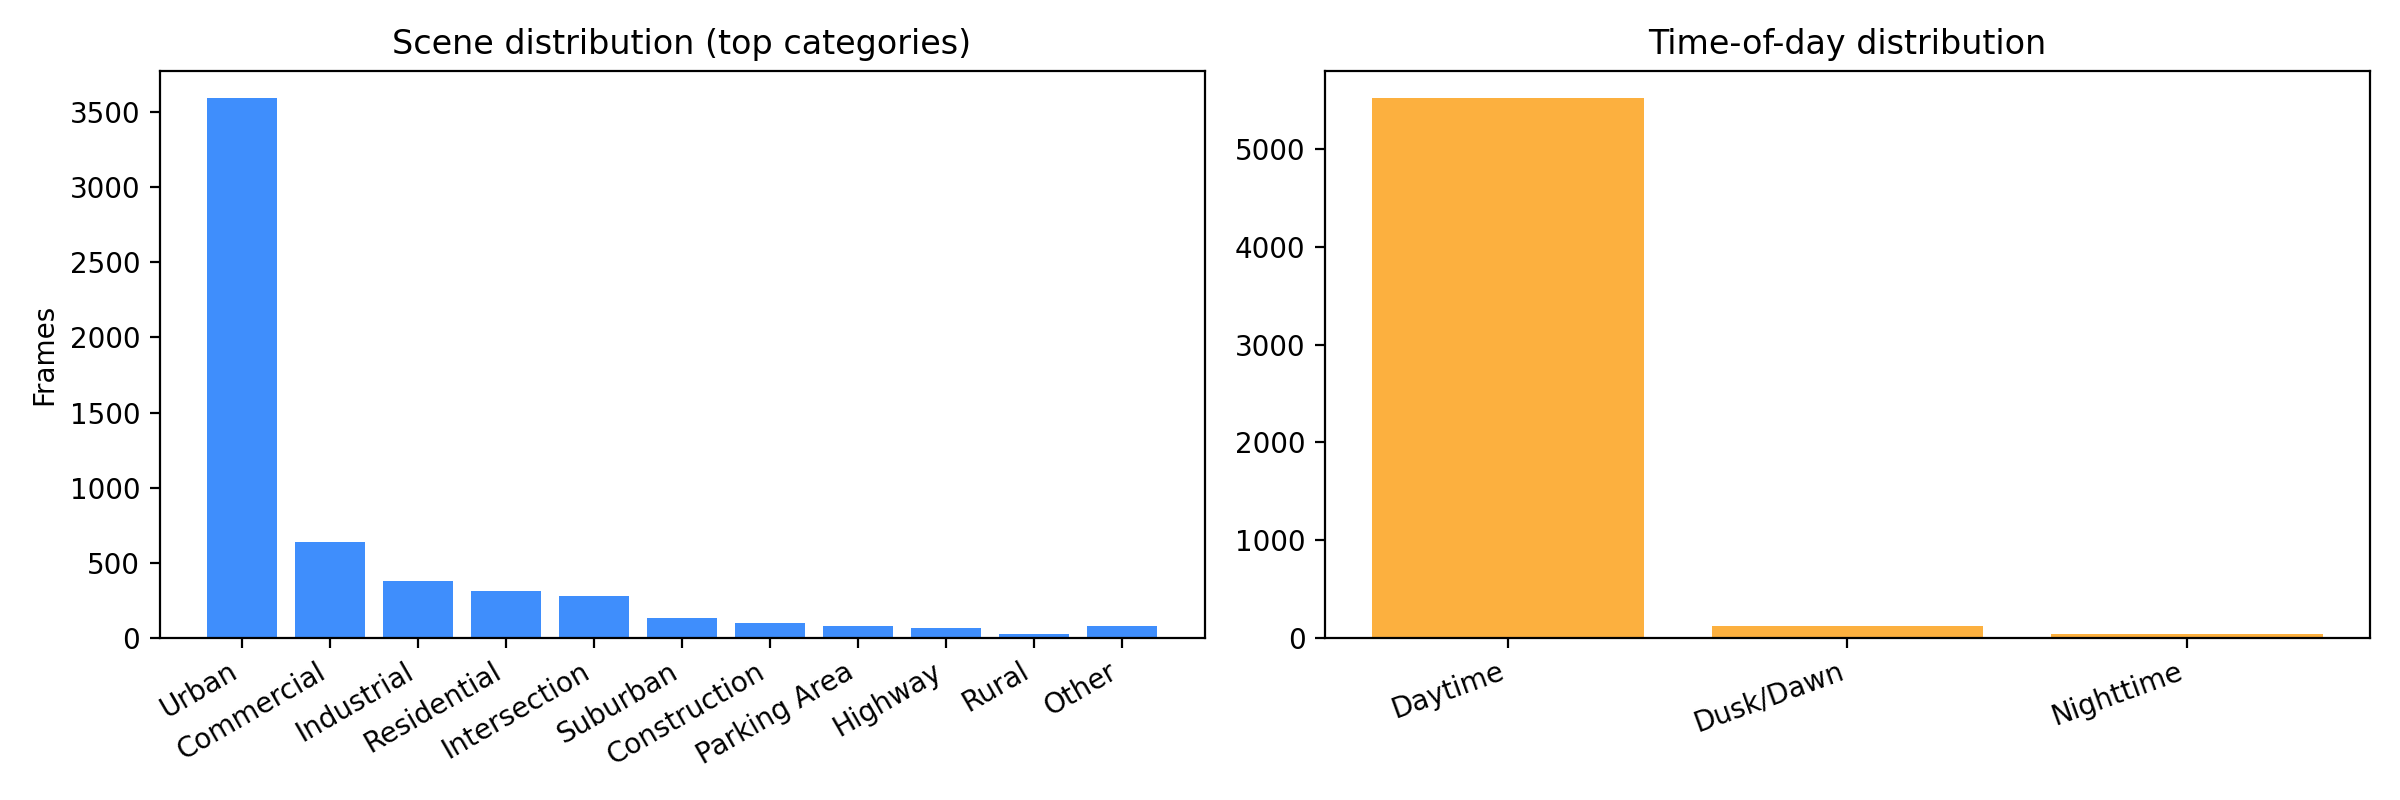
\includegraphics[width=\linewidth]{figs/dataset_attribute_distribution.png}
    \caption{Dataset attribute distribution for representative benchmark fields, including weather, traffic-light state, and vehicle-count marginals.}
    \label{fig:dataset-attributes}
\end{figure*}

\begin{figure}[t]
    \centering
    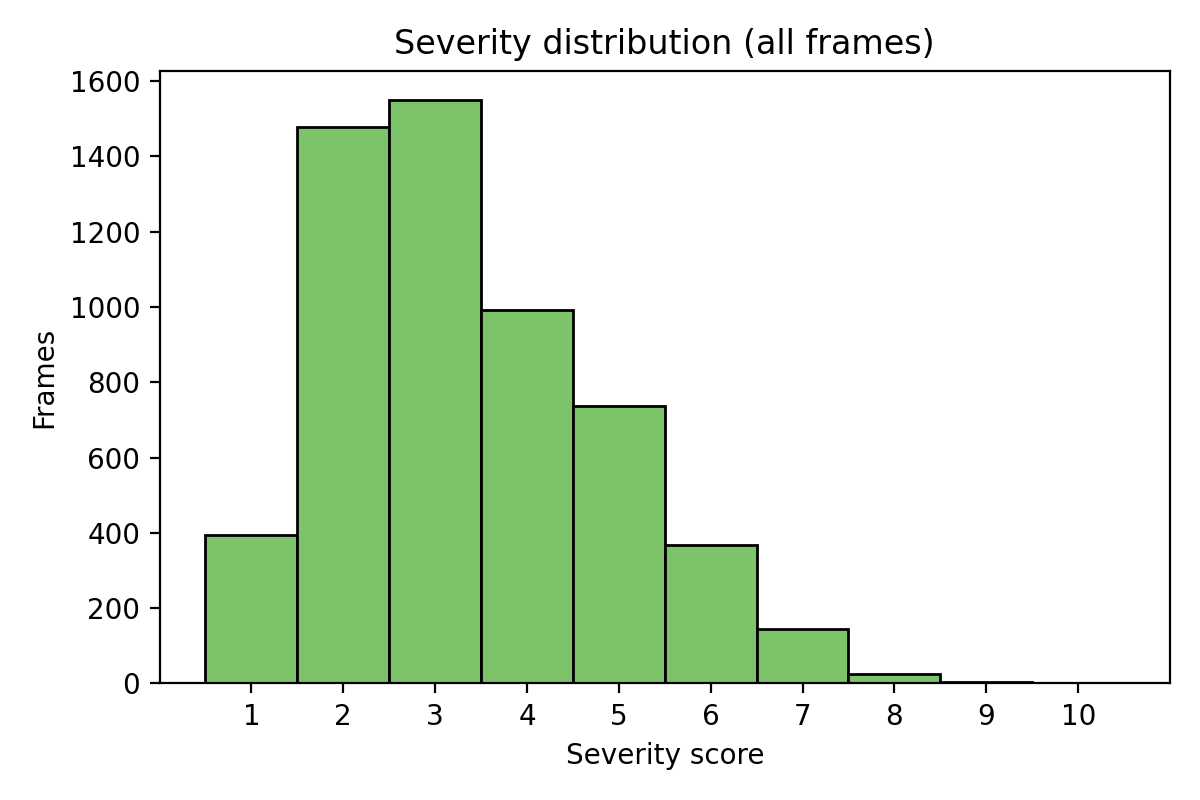
\includegraphics[width=\linewidth]{figs/dataset_severity_histogram.png}
    \caption{Severity histogram over the full canonical release.}
    \label{fig:dataset-severity}
\end{figure}

\subsection{Scenario Coverage}
The full release contains \textbf{5,032} daytime scenes, \textbf{111} dusk/dawn scenes, and \textbf{39} nighttime scenes. It also contains \textbf{1,586} scenes with visible traffic lights, \textbf{1,781} scenes with vulnerable road users, and \textbf{2,552} scenes tagged as adverse-condition cases by the benchmark slice helper fields. These counts clarify two points raised in the IV reviews: the corpus is intentionally heterogeneous but not balanced, and meaningful scenario mining requires reporting support counts alongside accuracy or F1.

\subsection{Release QA}
The release builder performs three types of checks before emitting the canonical JSONL file:
\begin{itemize}
  \item \textbf{Record alignment}: image basenames and label basenames must match within each source dataset.
  \item \textbf{Schema normalization}: enum drift, misplaced fields, and optional legacy keys are normalized into the benchmark schema.
  \item \textbf{Split validation}: every split manifest must point to existing canonical records and no train/dev/audit overlap is allowed.
\end{itemize}

In the current snapshot, the canonicalizer recovers \textbf{5,192} usable records, skips \textbf{3} images without matching raw labels, and ignores \textbf{2} extra raw labels without matching images. The release logger also records normalization actions for recurrent drift patterns such as misplaced vehicle-type labels inside the traffic-sign object and spelling or formatting variants in categorical fields. These structural normalization steps operate on records that have already been manually reviewed and corrected; they should not be interpreted as replacing human annotation with automatic post-processing.

\subsection{Coverage Notes}
CARScenes is intentionally heterogeneous but not perfectly balanced. Daytime scenes dominate the release, high-severity scenes are rare, and the four source datasets contribute different mixtures of road geometry and traffic control. We therefore recommend reporting both overall metrics and slice metrics. In particular, traffic-light state should only be scored where the field is present, and slices that depend on higher severity or adverse visibility should be reported with support counts alongside accuracy or F1.

\subsection{Limitations}
CARScenes remains a single-frame benchmark. Temporal ambiguity affects some fields more than others, especially \texttt{Ego-Vehicle.Direction}, \texttt{Ego-Vehicle.Maneuver}, \texttt{Vehicles.States}, and event-level \texttt{Severity} judgments. Interactive demos built on top of these labels should therefore be treated as illustrative rather than authoritative; without human correction, a VLM can hallucinate lanes, actor states, or traffic control. The released corpus is fully human-corrected, but the current paper does not report corpus-wide inter-annotator agreement because the full correction pass was performed by a primary annotator rather than by multiple independent annotators. Finally, the benchmark evaluates scene understanding and failure slicing; it does not evaluate a downstream driving policy.

\subsection{Licensing}
CARScenes combines our own annotations, schema, and benchmark code with upstream image identifiers from Cityscapes, KITTI, Argoverse1, and nuScenes. Our release artifacts are annotation-only and do not re-license the original images. Users must obtain the source images under the original dataset terms, cite the upstream datasets alongside CARScenes, and treat the original corpora as dependencies rather than as newly released data in this submission.
